\documentclass[12pt,twoside,a4paper]{article}
\renewcommand*\familydefault{\sfdefault}
\usepackage[utf8]{inputenc}
\usepackage[T1]{fontenc}
\usepackage[ngerman]{babel}
\usepackage[left=3cm,right=3cm,top=2cm,bottom=4cm]{geometry}
\usepackage{graphicx}
\usepackage{helvet}
\renewcommand{\familydefault}{\sfdefault}
\linespread{1.25}
\usepackage[table]{xcolor}
\usepackage{hyperref}
\hypersetup{
    colorlinks,
    linkcolor={black!},
    citecolor={blue!50!black},
    urlcolor={blue!50!black}
}
\definecolor{light-yellow}{RGB}{255, 255, 204}
\usepackage[numbib,nottoc]{tocbibind}
\usepackage{caption}
\usepackage{fancyvrb}
\usepackage{graphicx}
\usepackage{apacite}
\usepackage[acronym]{glossaries}
\makeglossaries
\newacronym{erm}{ERM}{Entity Relationship Model}
\newacronym{uml}{UML}{Unified Markup Language}
\newacronym{jakarta-ee}{Jakarta EE}{Jakarta Enterprise Edition}
\newacronym{cdi}{CDI}{Context Dependency Injection}
\newacronym{iata}{IATA}{IATA airport code}
\newacronym{ci}{CI}{Continuous Integration}
\newacronym{jar}{JAR}{Java Archive}
\newacronym{war}{WAR}{Web Application Resource}
\newacronym{ejb}{EJB}{Enterprise JavaBeans}
\begin{document}
\pagenumbering{gobble}
% Deckblatt
\begin{center}
\href{https://www.intension.de/}{
\includegraphics[width=6cm]{images/intension}}\hfill\href{https://www.dhbw-stuttgart.de}{
\includegraphics[width=4cm]{images/dhbw}}\\
\large
\vspace{3cm}
\textbf{Featherkraken}: Bestpreissuche für Flugangebote mit variablen Abflughäfen\\
\vspace{2cm}

\includegraphics[width=4cm]{images/featherkraken}\\
\textbf{\Large STUDIENARBEIT}
\vspace{1cm}
\\des Studienganges Informatik
\\an der Dualen Hochschule Baden-Württemberg Stuttgart
\\von
\\Ingo Kuba
\end{center}
\vfill
\textbf{Matrikelnummer, Kurs}\hfill place, holder\\
\textbf{Ausbildungsfirma}\hfill intension GmbH\\
\textbf{Betreuer}\hfill Place Holder
\newpage
% Pre-Einleitung
\section*{Erklärung zur Eigenleistung}
Hiermit erkläre ich, dass ich die vorliegende Studienarbeit selbständig verfasst und keine anderen als die angegebenen Hilfsmittel benutzt habe.\\
Die Stellen der Studienarbeit, die anderen Quellen im Wortlaut oder dem Sinn nach entnommen wurden, sind durch Angaben der Herkunft kenntlich gemacht. Dies gilt auch für Zeichnungen, Skizzen, bildliche Darstellungen sowie für Quellen aus dem Internet.
\vspace{1cm}\\Ostfildern, den \today \hspace{1cm} \hrulefill
\newpage
% Abstract
\begin{sloppypar}
\section*{Zusammenfassung}
Bei Flügen über lange Strecken ist es häufig günstiger, Routen über nahe gelegene Flughäfen zu buchen. Um diese alternativen Routen zu finden, bieten Flugsuchdienste oft nur die Eingabe mehrerer Flughäfen an. Da diese für Reisende nicht alle bekannt sein können, wäre es besser einen Radius um den geplanten Abreiseort angeben zu können. Die Suchmaschine sucht darin nach Flughäfen und ermittelt Flüge von diesen zum Ziel.\\
Im Rahmen dieser Studienarbeit wurde eine Softwarelösung entwickelt, welche diese Funktionalität in Form einer Webanwendung umsetzt.
\section*{Abstract}
For long flights, it is often cheaper to book routes via nearby airports. To find these alternative routes, flight booking services often only offer the entry of multiple airports. As travellers may not know all of them, it would be better to enter a radius around the planned departure location. The search engine will then search for airports in the given radius and find flights from these airports to the destination.\\
In the context of this study thesis a software solution was developed, which implements this functionality in form of a web application.
% Verzeichnisse
\newpage
\tableofcontents
\newpage
\listoffigures
\vfill
\printglossary[type=\acronymtype]
\newpage
\interlinepenalty=10000
\pagenumbering{arabic}
\setcounter{page}{1}
% Einleitung:
\section{Einleitung}
\subsection{Motivation}
In der Regel möchte ein Fluggast den günstigsten Preis für eine bestimmte Route von A nach B. Jede Flugsuchmaschine im Internet bietet dieses Feature. Manchmal sucht ein Fluggast auch einfach nach Inspiration und möchte Angebote von A nach X, wobei X variabel ist. Einige Suchmaschinen bieten diese Suche ebenfalls bereits an. Worum es in dieser Studienarbeit geht, ist der umgekehrte Fall: X nach B. Also von welchem beliebigen Flughafen man möglich günstig an ein festes Ziel kommt. Gerade auf hochpreisigen Strecken kann es sich lohnen einen Umweg zu fliegen.
\subsection{Aufgabenstellung}\label{sec:requirements}
Bei der Suche sollen die klassischen Filterkriterien implementiert werden, welche als Pflichtanforderungen bezeichnet werden. Das heißt die Unterscheidung ob man nur einen Hinflug oder Hin- und Rückflug buchen möchte. Des Weiteren soll man jeweils ein Datum für An- und Abreise festlegen können, welches um drei Tage flexibel sein soll. Neben der Buchungsklasse (Economy, Business, First Class) soll auch die Wahl der Airline oder Allianz eingeschränkt werden können. Außerdem soll man Passagier- und Umsteigeanzahl wählen können.\newline
Zusätzlich soll ein Entfernungsfilter um einen möglichen Abflughafen bereitgestellt werden. Zum Beispiel wird nur nach Angeboten gesucht, bei dem sich der Startflughafen maximal 800km (Entfernungsfilter) vom Flughafen Stuttgart (möglicher Abflughafen) entfernt befindet.\newline
Diese Flugsuchmaschine soll über ein Web-Frontend vom Nutzer bedient werden können.
\newpage
\section{Wissenschaftliche Vertiefung}
In diesem Kapitel werden technische Grundlagen aufgeführt und erläutert, welche für die Entwicklung des Projekts benötigt wurden.
\subsection{Entity Relationship Model}
Um das Datenmodell der Anwendung darzustellen wurde eine vereinfachte Variante des \acrfull{erm} verwendet. Hier werden zunächst nur die Grundlagen zu dieser Modellvariante beschrieben ohne auf das eigentliche Datenmodell einzugehen, welches dann in Kapitel \ref{sec:data-model} vorgestellt wird.
\subsection*{Entities}
Ein Objekt oder auch Entity wird in einem Rechteck dargestellt und kann Attribute besitzen, wobei komplexe Attribute als Beziehungen zu anderen Objekten dargestellt werden. Der Name der Beziehung entspricht hierbei dem Attributnamen. Die Anzahl der möglichen Relationen wird in \acrshort{uml}-Notation angegeben. Zum Beispiel ist hier in Abbildung \ref{fig:erm-entity} zu sehen, dass eine Person null bis n Autos besitzen kann.
\begin{center}
	\captionsetup{type=figure}
	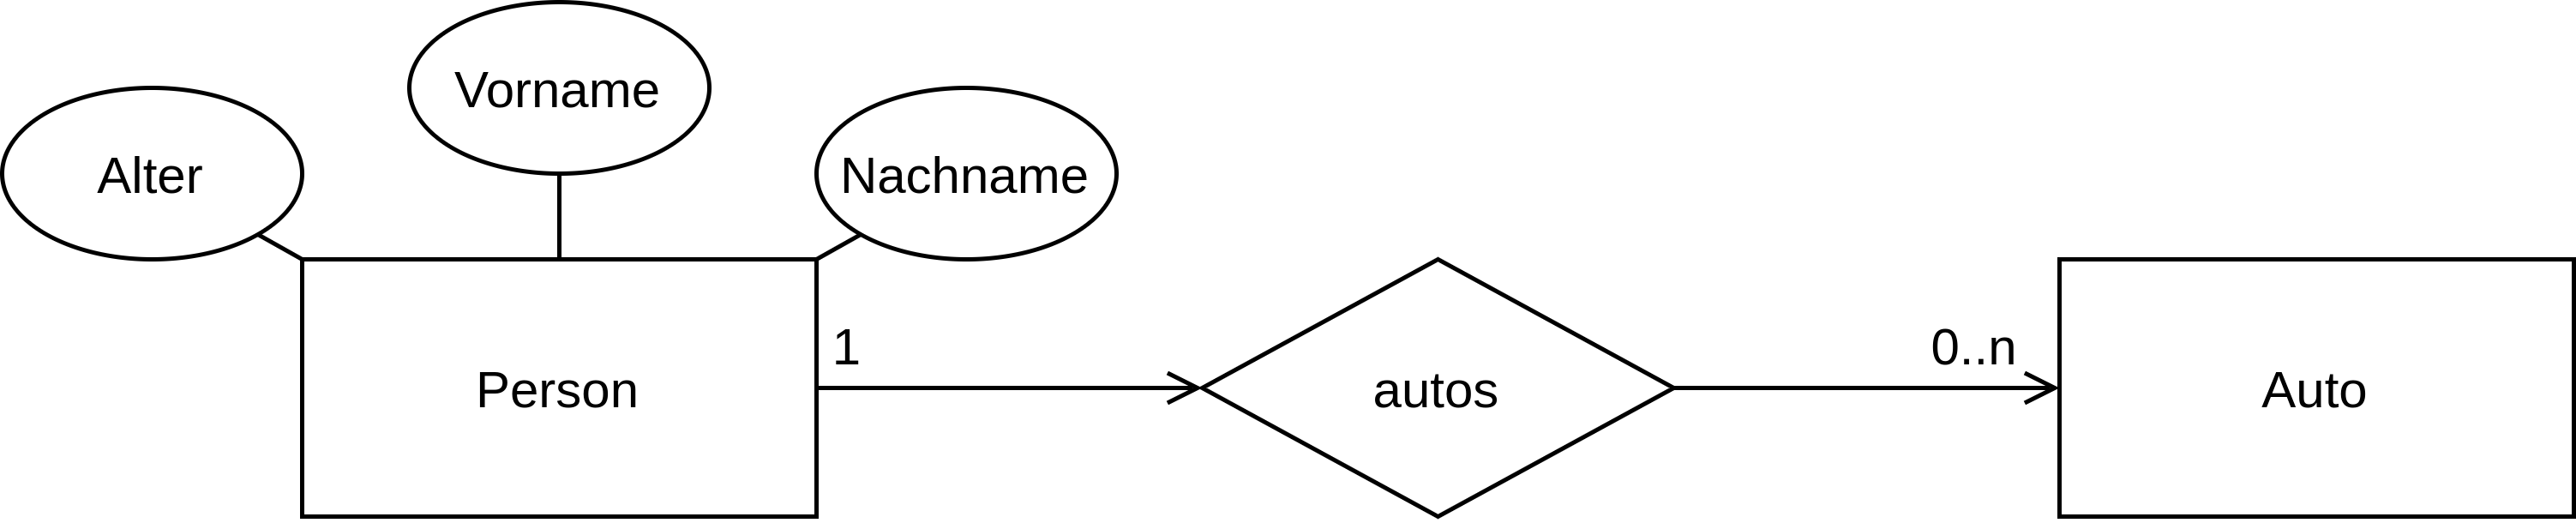
\includegraphics[width=\textwidth]{images/ERM-Entity}
	\captionof{figure}[Beispiel für eine Entity im \acrshort{erm}]{Beispiel für eine Entity mit Attributen und einer Beziehung}
	\label{fig:erm-entity}
\end{center}
\subsection*{Attribute}
Attribute können dabei eindeutig, optional oder mehrwertig sein. Die Unterscheidung zwischen Datum, Zahl oder Zeichenkette wird dabei in einem \acrlong{erm} nicht dargestellt.
\begin{center}
	\captionsetup{type=figure}
	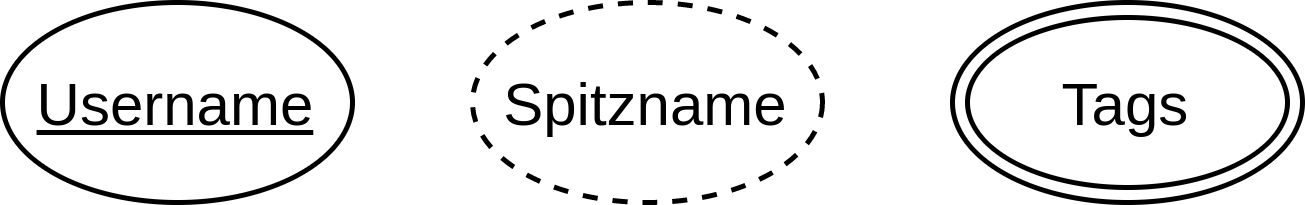
\includegraphics[width=10cm]{images/ERM-Attributes}
	\captionof{figure}[Verschiedene Arten von Attributen im \acrshort{erm}]{Attribute (v.l.): eindeutig, optional und mehrwertig}
	\label{fig:erm-attributes}
\end{center}
\subsection{Docker}
Docker ist eine quelloffene Software zur Isolierung von Anwendungen in sogenannten Containern. Mit ihr können zum Beispiel Webserver oder Datenbanken schnell eingerichtet werden, ohne diese vorher aufsetzen zu müssen.
\subsubsection{Image}
\textit{Images} sind die Vorlage zur Erstellung neuer Container. Sie können aus mehreren Schichten von anderen Images bestehen und so können komplexe Systeme leichtgewichtig und portabel erstellt werden.
\subsubsection{Container}
Ein \textit{Container} ist die aktive Instanz eines Docker images und kann beliebig konfiguriert und bearbeitet werden. Wird ein Container beendet und ein neuer nach der Vorlage desselben Images gestartet, gehen alle Änderungen verloren. Dies lässt sich durch die Verwendung von \textit{Volumes} verhindern, welche die Konfiguration eines Containers persistieren.
\subsection{Git}
Git ist eine kostenlose Softwarelösung zur verteilten Versions-Verwaltung von Dateien und eignet sich ideal für Softwareprojekte. Git wurde 2005 von Linus Torvalds entwickelt, welcher als der Erfinder von Linux gilt. \cite{linus-torvalds}\\
Versionen eines Projekts werden dabei in sogenannten \textit{commits} festgehalten. Außerdem gibt es \textit{branches} um verschiedene Entwicklungsstände zu repräsentieren. Dabei gibt es immer einen Branch mit der aktuell validen Version des Projekts (meistens '\textit{master'}). Dateiänderungen können zwischen verschiedenen Branches ausgetauscht werden, wobei hauptsächlich der Befehl \textit{merge} benutzt wird um Änderungen auf den \textit{master}-Branch zu erhalten.\\
Das Projekt befindet sich in einem lokalen \textit{repository} auf dem Computer des Bearbeiters, aber kann auch mit einem Repository im Internet synchronisiert werden. Um Änderungen vom lokalen Repository in das Webrepository zu veröffentlichen wird der Befehl \textit{push} benutzt. Für den umgekehrten Fall (also Internet $\rightarrow$ Lokal) wird der Befehl \textit{pull} verwendet.
\subsubsection{GitHub}
Ein kostenloser Anbieter für ein Webrepository ist zum Beispiel \href{https://github.com/}{\textit{GitHub}}, welches dabei am bekanntesten ist. Neben einer Weboberfläche zum Verwalten der Branches bietet GitHub unter anderem Verwaltung von Zugriffsrechten, Aufgabenorganisation und eine eingebaute \acrshort{ci}.\\
Um Änderungen zwischen Branches auszutauschen bietet GitHub sogenannte \textit{pull requests}. In diesen werden die Änderungen übersichtich dargestellt und ein akzeptieren des Pull Request hat einen \textit{merge} in den Ziel-Branch zur Folge.\\
Die Aufgabenorganisation wird mithilfe von \textit{Issues} durchgeführt, welche sich zusammensetzen aus Titel, Beschreibung und Metadaten wie Bearbeitender, Label oder Bearbeitungsstatus. Der Bearbeitungsstatus der Issues lässt sich in einem \textit{Project}-Board (zum Beispiel Kanban/Scrum) organisieren.\\
Des Weiteren bietet \textit{GitHub Pages} die Möglichkeit, kostenlos statische Web-Inhalte zu hosten. Dabei kann eine \acrshort{ci} benutzt werden um die Inhalte aus dem jeweiligen Projekt automatisch zu generieren und veröffentlichen.\\
Auf GitHub befinden sich für diese Studienarbeit sowohl die \href{https://github.com/featherkraken}{Repositories} als auch das automatisierte \href{https://github.com/orgs/featherkraken/projects/1}{Project-Board} dazu. Außerdem wurden die aktuelle Versionen des \href{https://featherkraken.github.io/featherkraken-ui/}{Frontends} und dieses \href{https://featherkraken.github.io/featherkraken-paper/paper.pdf}{Dokuments} in GitHub Pages veröffentlicht.
\subsection{CircleCI}
Da die eingebaute \acrshort{ci} von GitHub nicht zufriedenstellend mit Docker zusammen funktioniert, wurde die externe Lösung \href{https://circleci.com/}{CircleCI} verwendet. Dabei lassen sich Docker-Container zum Ausführen von Befehlen verwenden um komplexere Szenarien umsetzen zu können. Die gute Integration von GitHub und CircleCI hat zur Folge, dass Tests und andere Überprüfungen automatisch mit jedem \textit{push} ausgelöst werden können. Diese Überprüfungen lassen sich im \textit{pull request} des betroffenen Branches nachvollziehen und auftretende Fehler werden sofort dargestellt.
\subsection{Maven}
Maven ist ein Management-Tool für Softwareprojekte und wird dabei hauptsächlich für Java-Projekte verwendet. Die Konfiguration des Projekts befindet sich in einem XML-Dokument (standardmäßig \textit{pom.xml}), in dem Bibliotheken und Plugins verwaltet werden. Mit Maven lässt sich ein ausführbares Artefakt des Projekts bauen, zum Beispiel als \acrfull{jar}, \acrfull{war} oder \acrfull{ejb}.\newline\cite{maven-packaging}
\subsubsection{Ordnerstruktur}
Maven zeichnet sich durch eine bestimmte Ordnerstruktur aus, welche strikt eingehalten werden muss.\\
\texttt{src/main/java} Enthält die Java-Klassen für die Funktion des Projekts.\\
\texttt{src/main/resources} Enthält Ressourcen für die Funktion des Projekts.\\
\texttt{src/test/java} Enthält die Java-Klassen für Software-Tests.\\
\texttt{src/test/resources} Enthält Ressourcen für die Software-Tests.\\
Darüber hinaus gibt es noch weitere Ordner für spezielle Zwecke.\newline\cite{maven-dir-layout}
\subsubsection{Dependencies}
Externe Bibliotheken lassen sich leicht als \textit{dependency} einbinden, wobei die jeweiligen Artefakte aus Maven-Repositories im Internet heruntergeladen werden. Eine Dependency wird eindeutig durch Gruppen-ID (\texttt{groupId}), Artefakt-ID (\texttt{artifactId}) und Version (\texttt{version}) definiert. So wird sichergestellt, dass immer die gewünschte Bibliothek benutzt wird.
\subsubsection{Plugins}
Um verschiedene Befehle auf dem Projekt auszuführen, können Plugins verwendet werden. Diese lassen sich mit den gewünschten Parametern konfigurieren, um zum Beispiel Unit- und Integrations-Tests auszuführen oder die Testabdeckung dessen zu überprüfen.
\subsection{\acrshort{jakarta-ee}}\label{sec:jakarta-ee}
\acrfull{jakarta-ee} ist eine Java-Spezifikation, welche Java SE (Standard Edition) erweitert und ermöglicht damit das Entwickeln von mehrschichtigen, zuverlässigen und sicheren Netzwerkanwendungen. Zuvor war \acrshort{jakarta-ee} als Java EE bekannt.\newline\cite{java-ee}
\subsection{MicroProfile}\label{sec:microprofile}
Eclipse MicroProfile ist eine Erweiterung von \acrshort{jakarta-ee} und eine Alternative zu Spring, welches ein Framework der Firma Pivotal und vielgenutzte Lösung für \acrshort{jakarta-ee} Anwendungen und Microservices ist.\newline
MicroProfile bietet hingegen unter anderem Unterstützung für \acrfull{cdi}, sowie eine bessere Konfigurierbarkeit der Anwendung.\newline\cite{microprofile}
\subsection{Payara}
Payara ist ein Application Server für Java-Anwendungen, insbesondere \acrshort{jakarta-ee}. Ein Application Server führt Anwendungsprogramme aus und bietet zum Beispiel Dienste für Restschnittstellen, Authentifizierung oder Datenbankzugriff. \cite{app-server}\newline
Payara basiert auf dem GlassFish Server, erweitert diesen jedoch um besseren Support sowie regelmäßigere Releases und Sicherheitsupdates.\newline\cite{payara-vs-glassfish}
\subsection{Postman}\label{sec:postman}
Postman ist ein Programm um HTTP-Schnittstellen aufzurufen um diese zu testen. Die einzelnen Aufrufe können in sogenannten \textit{Collections} in Json-Format gespeichert werden, sodass sie in einer anderen Postman-Instanz importiert und wiederverwendet werden können. Durch diese beispielhaften Aufrufe ist es einfach, den Aufbau einer Schnittstelle zu verstehen.
\subsection{React.js}\label{sec:react}
React.js ist eine JavaScript-Bibliothek um Webanwendungen zu entwickeln. Damit lassen sich einfach interaktive Oberflächen erstellen, wobei man für jede Komponente der Anwendung sogenannte \textit{Views} definiert. Dabei rendert React.js eine Komponente nur neu, wenn sich dessen Daten ändern. Dadurch wird die Anwendung effizient und der Code wird übersichtlicher und einfacher zu debuggen. Außerdem lassen sich Komponenten abstrakt definieren und mehrfach verwenden, was der gesamten Anwendung ein einheitliches Aussehen gibt. \cite{react}
\subsection{TypeScript}\label{sec:typescript}
TypeScript ist eine auf JavaScript basierende Programmiersprache und erweitert diese um viele Funktionen aus der objektorientierten Programmierung. Der geschriebene Code wird zu JavaScript kompiliert, dadurch sind auch Bibliotheken und Syntax von JavaScript einsetzbar. Ein großer Vorteil gegenüber JavaScript ist, dass TypeScript strikter sein kann und somit logischer und verständlicher Code entsteht. \cite{ts-vs-js}
\newpage
% Hauptteil
\section{Entwurf}
In diesem Kapitel werden Ansätze zur Implementierung der Anwendung verglichen und die jeweils gewählte Lösung aufgeführt. Die Ansätze reichen durch alle Abstraktionsebenen von Überlegungen zum Aufbau des Projekts, über Modellierung der Daten bis hin zu gewählten Frameworks.
\subsection{Auswahl der externen Schnittstelle}
Um Flugdaten zu erhalten muss eine externe Schnittstelle benutzt werden, welche die Pflichtanforderungen\textsuperscript{\ref{sec:requirements}} erfüllt und dabei leicht zu verwenden ist. Die Wahl der Schnittstelle fiel dabei auf eine Rest-Schnittstelle, da diese sehr einfach zu benutzen sind. Für die Auswahl des Anbieters wurde eine Tabelle (siehe Abbildung \ref{fig:api-comparison}) erstellt, welche die Pflichtanforderungen mit den Funktionalitäten der jeweiligen Schnittstelle abgleicht. Dabei erfüllte die Schnittstelle von Kiwi nicht nur alle Anforderungen, sondern war auch sehr gut dokumentiert und mit Beispielen beschrieben. Des Weiteren bot Kiwi auch eine Rest-Schnittstelle um Flughäfen mit Teilen des Städte- oder Flughafennamens und in einem Radius um bestimmte Koordinaten zu suchen, was der Aufgabenstellung entgegen kam.
\begin{center}
	\captionsetup{type=figure}
	\resizebox{\textwidth}{!}
	{\begin{tabular}{ l | c | c | c | c | c | c }
			& \textbf{Skyscanner} & \textbf{Hipmunk} & \textbf{Kajak} & \textbf{Flight Data} & \textbf{Flight Bookings} & \textbf{Kiwi Flights}\\
			\hline
			\textbf{Single flight} & \cellcolor{green!50}yes & \cellcolor{green!50}yes & \cellcolor{green!50}yes & \cellcolor{green!50}yes & \cellcolor{green!50}yes & \cellcolor{green!50}yes\\
			\hline
			\textbf{Two directions} & \cellcolor{red!75}no & \cellcolor{red!75}no & \cellcolor{red!75}no & \cellcolor{green!50}yes & \cellcolor{red!75}no & \cellcolor{green!50}yes\\
			\hline
			& & & & & &\\
			\hline
			\textbf{Specific date} & \cellcolor{green!50}yes & \cellcolor{green!50}yes & \cellcolor{green!50}yes & \cellcolor{green!50}yes & \cellcolor{green!50}yes & \cellcolor{green!50}yes\\
			\hline
			\textbf{Flexible date} & \cellcolor{red!75}no & \cellcolor{yellow!75}limited & \cellcolor{yellow!75}limited & \cellcolor{green!50}yes & \cellcolor{red!75}no & \cellcolor{green!50}yes\\
			\hline
			& & & & & &\\
			\hline
			\textbf{Class} & \cellcolor{green!50}yes & \cellcolor{green!50}yes & \cellcolor{green!50}yes & \cellcolor{yellow!75}limited & \cellcolor{green!50}yes & \cellcolor{green!50}yes\\
			\hline
			\textbf{Passengers} & \cellcolor{green!50}yes & \cellcolor{green!50}yes & \cellcolor{green!50}yes & \cellcolor{red!75}no & \cellcolor{green!50}yes & \cellcolor{green!50}yes\\
			\hline
			\textbf{Airline} & \cellcolor{green!50}yes & \cellcolor{red!75}no & \cellcolor{red!75}no & \cellcolor{red!75}no & \cellcolor{red!75}no & \cellcolor{green!50}yes\\
			\hline
			\textbf{Stops} & \cellcolor{red!75}no & \cellcolor{red!75}no & \cellcolor{red!75}no & \cellcolor{red!75}no & \cellcolor{red!75}no & \cellcolor{green!50}yes
	\end{tabular}}
	\captionof{figure}[Vergleich der Schnittstellen]{Tabelle zum Vergleich der Schnittstellen}
	\label{fig:api-comparison}
\end{center}
\subsection{Aufbau der Anwendung}
Bei dem ersten Entwurf der Anwendung fiel auf, dass die gesamte Funktionalität mit zwei verschiedene Ansätzen gelöst werden kann. Zum einen könnte man externe Schnittstellen direkt aus dem Frontend aufrufen, sodass eine Serveranwendung nicht notwendig wäre. Dies hätte den Vorteil, dass der Technologie-Stack reduziert würde. Andererseits hätte es den Nachteil, dass das Projekt unübersichtlich werden könnte. Deshalb ist es sinnvoll, ein clientseitiges User Interface und eine separate Serveranwendung für die Funktionalität zu entwickeln und jeweils passende Technologien für beide zu finden.
\begin{center}
	\captionsetup{type=figure}
	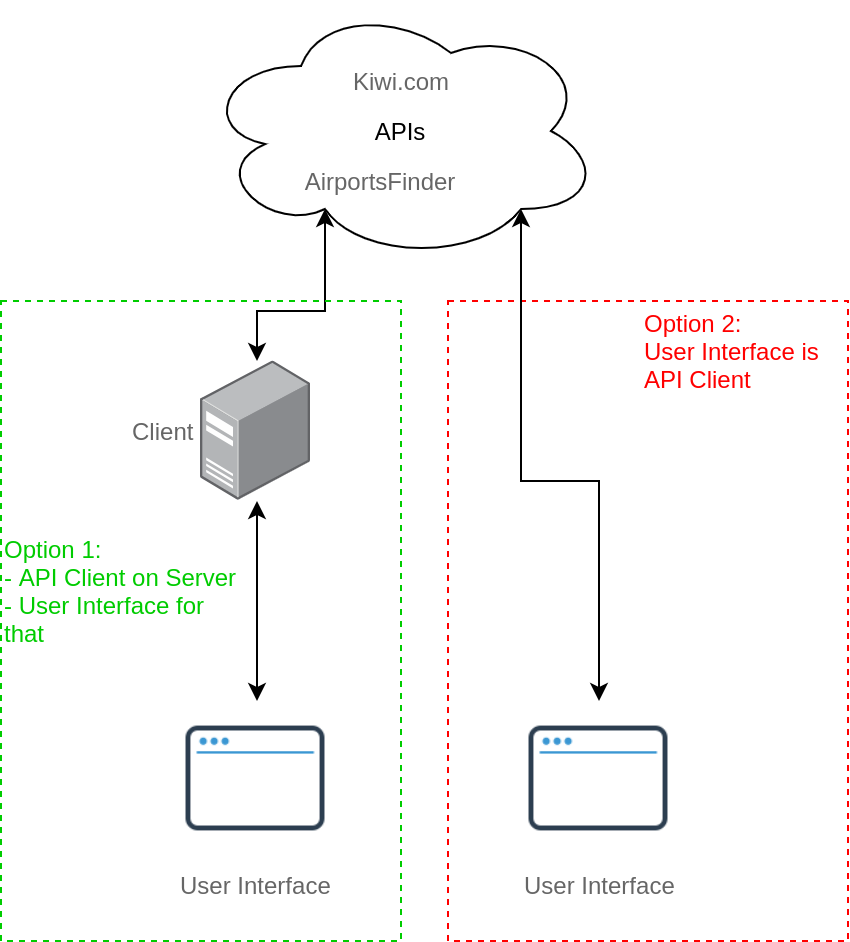
\includegraphics[width=7cm]{images/client-design}
	\captionof{figure}[Aufbau der Anwendung]{Aufbau der Anwendung}
\end{center}
\subsection{Datenmodell}\label{sec:data-model}
Das \acrlong{erm} für das Datenmodell wurde hier aufgeteilt in Suchanfrage (\texttt{SearchRequest}) und Suchergebnis (\texttt{SearchResult}). Sowohl die Serveranwendung als auch das User Interface implementieren jeweils dieses Datenmodell, sodass Daten in einem einheitlichen und überschaubaren Format ausgetauscht werden können.
\subsubsection{SearchRequest}
Eingehende Anfragen an den Service (\texttt{SearchRequest}) haben verschiedene Parameter, welche die zu Beginn genannten Pflichtanforderungen\textsuperscript{\ref{sec:requirements}} abdecken. Komplexe Attribute wie die Zeitspanne (\texttt{Timespan}) für An- und Abreise sowie der Ursprungs- und Ziel-Flughafen (\texttt{Airport}) wurden in eigene Objekte ausgelagert, damit sie so wiederverwendet werden können.
\begin{center}
	\captionsetup{type=figure}
	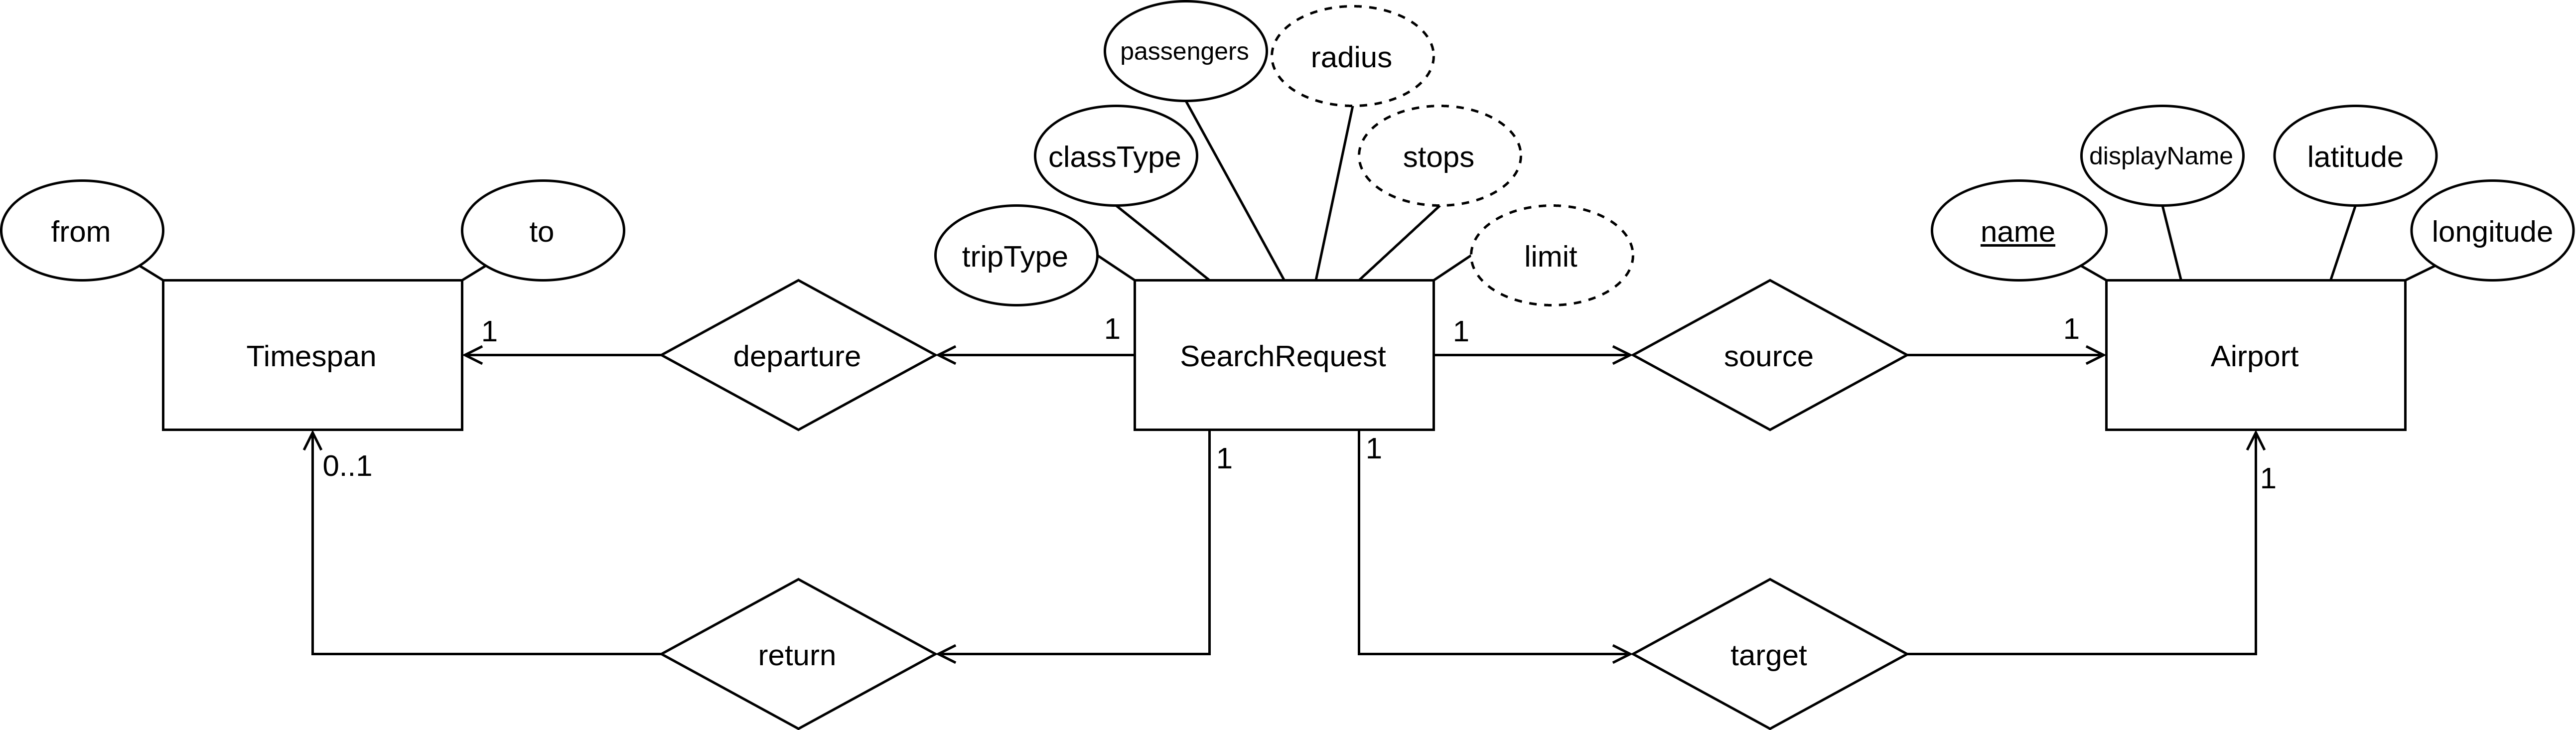
\includegraphics[width=\textwidth]{images/datamodel-SearchRequest}
	\captionof{figure}[\acrshort{erm} SearchRequest]{\acrlong{erm} des SearchRequest Objekts}
\end{center}
\subsubsection{SearchResult}
Antworten des Service (\texttt{SearchResult}) sind etwas komplexer als Anfragen aufgebaut, teilen jedoch manche Attribute mit diesen. So enthält ein Suchergebnis eine Ansammlung von sogenannten \texttt{Trips}, welche sich aus Flügen (\texttt{Flight}) der An- und Abreise zusammensetzen. Diese Flügen haben widerrum selbstverständlich selbst jeweils einen Start- und Zielflughafen, welche in dem \texttt{Route}-Objekt mit Informationen zu Abflug- und Ankunftzeiten sowie der Airline enthalten sind.\\
Bei erster Betrachtung fällt auf, dass Informationen über Airlines und Zeiten redundant sind, was jedoch für die optimale Verarbeitung in der Oberfläche von Vorteil ist.
\begin{center}
	\captionsetup{type=figure}
	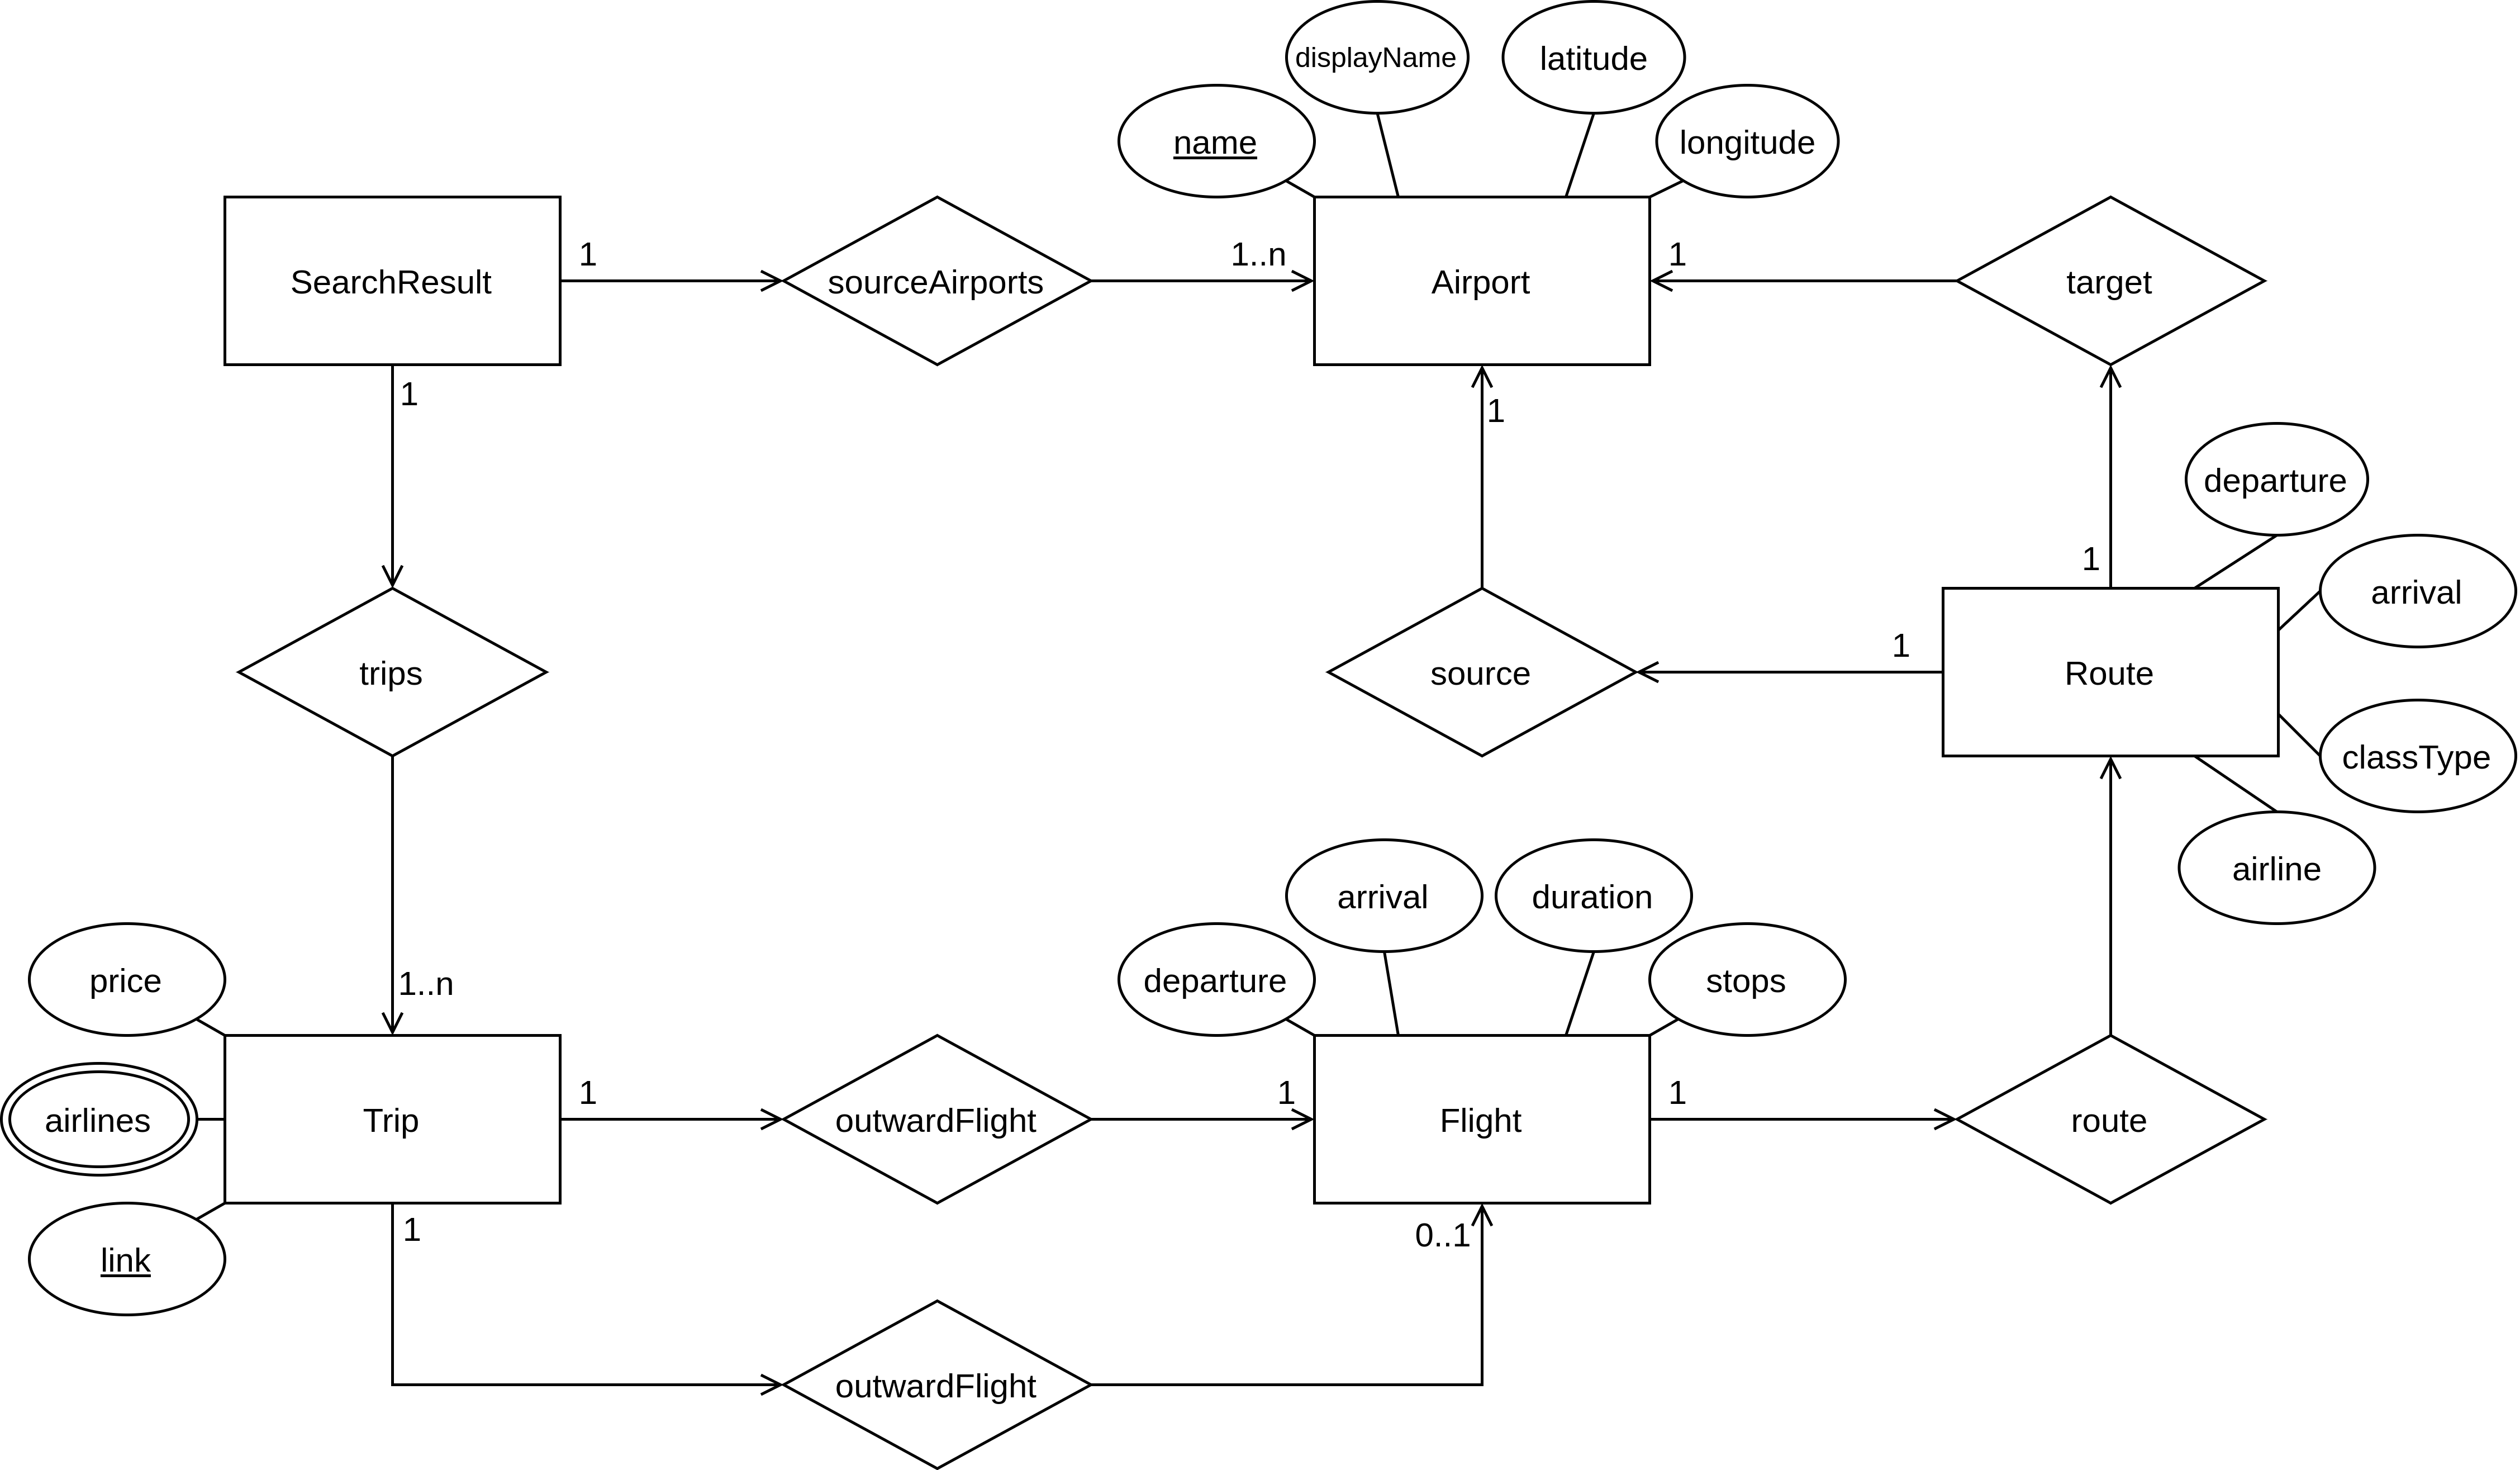
\includegraphics[width=\textwidth]{images/datamodel-SearchResult}
	\captionof{figure}[\acrshort{erm} SearchResult]{\acrlong{erm} des SearchResult Objekts}
\end{center}
\subsection{Framework}
Die Anwendung wurde in eine Server- und eine Web-Anwendung unterteilt, für welche jeweils eine Framework-Technologie gewählt werden muss. Die Serveranwendung übersetzt Suchanfragen von der Oberfläche zu einem Format, welches die externe Schnittstelle akzeptiert und leitet das Sucherergebnis daraufhin an die Oberfläche zurück. Dies bedeutet, dass die Serveranwendung als Rest-Client für die externe Schnittstelle und selbst als Rest-Schnittstelle für die Oberfläche dient.\\
Für die Komponenten war das Thema Plattformunabhängigkeit sehr wichtig und aus eigener Erfahrung eignet sich dafür Java sehr gut, da es eine große Community hat und eine Anwendung in kurzer Zeit aufgesetzt werden kann. Außerdem bietet Java einfache Möglichkeiten eine externe Rest-Schnittstelle anzusprechen.\\
Als Bedingung für die Web-Oberfläche ist es unabdingbar, dass die Anwendung intuitiv bedienbar ist und auf allen Endgeräten gut dargestellt werden kann. Als Programmiersprache wurde dabei JavaScript gewählt, aus denselben Gründen der Dokumentation und persönlicher Erfahrung. Dabei kommen drei bekannte Frameworks in Frage: Angular, React.js und Vue.js. Dabei wurde React.js gewählt, welches sich besser als Vue.js und Angular für kleine Anwendungen eignet, wie es in diesem Fall zutrifft. Bei dem hier vorliegenden Fall handelt es sich sogar um eine sogenannte Single-Page-Webapplication, das heißt die gesamte Funktion kann auf einer Webseite dargestellt werden.
\newpage
% Umsetzung
\section{Implementierung}
In diesem Kapitel wird die Umsetzung der Anwendung beschrieben. Wie bereits erwähnt, wurde die Anwendung in eine Serveranwendung (Backend) und eine Webanwendung (Frontend) unterteilt.
\subsection{Backend}
Das Backend der Anwendung dient als Proxy zwischen Frontend und externer Schnittstelle und wurde in Java geschrieben. Dabei wurde Jakarta EE\textsuperscript{\ref{sec:jakarta-ee}} und Eclipse Microprofile\textsuperscript{\ref{sec:microprofile}} verwendet, um eine Rest-Schnittstelle für das Frontend zu bieten. Durch das Verwenden von Microprofile lässt sich die Anwendung einfach in einem Payara Application Server starten. Dieser wurde mithilfe eines Docker Images umgesetzt, wodurch er sich einfach in einer Cloud Umgebung oder klassisch auf einem Windows- oder Linux-Server bereitstellen lässt.
\begin{center}
	\captionsetup{type=figure}
	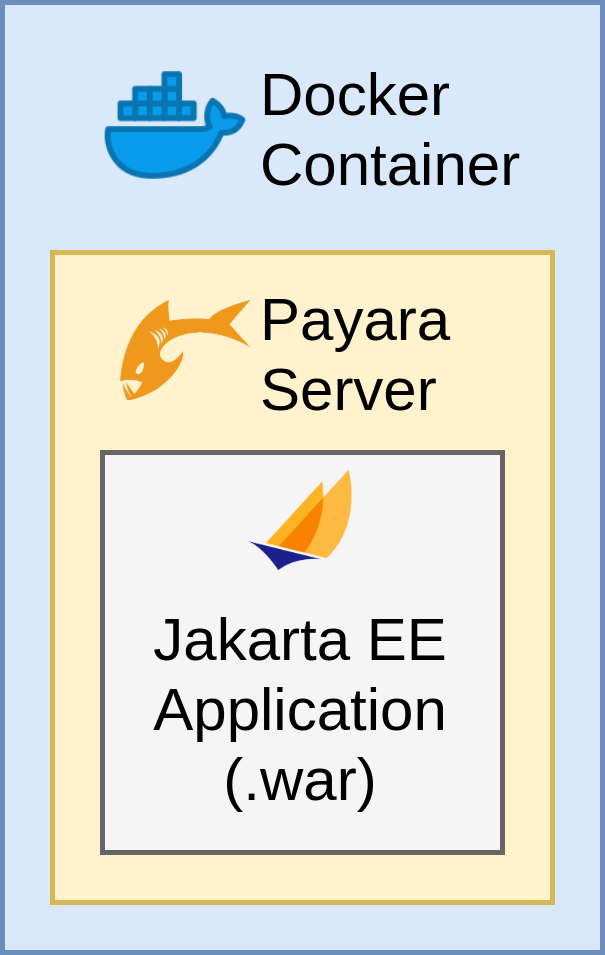
\includegraphics[height=5cm]{images/backend-structure}
	\captionof{figure}{Aufbau des Backends}
\end{center}
\subsubsection{Services}
Das Backend bietet verschiedene Rest-Services für ein User Interface, um nach Flughäfen und Flügen suchen zu können.
\paragraph[Flughafensuche]{Flughafensuche: GET /airports}\label{sec:airport-search}
Um bestimmte Flughäfen mit einem Teil des Flughafen- oder Städtenamens suchen zu können, gibt es den Endpoint \texttt{/airports} der mit einem GET-Request erreicht werden kann. Die Eingabe wird über den Query-Parameter 'query' in der URL des Requests übergeben. Ein beispielhafter Request für die Suche von Flughäfen in Amsterdam kann zum Beispiel folgendermaßen aufgebaut sein:\\
\begin{center}
	\texttt{GET www.featherkraken-example.com/airports?query=Ams}
\end{center}
Damit werden alle Flughäfen gesucht, welche den Wortteil 'Ams' im \acrlong{iata} oder Städtenamen enthalten. Die Antwort des Services besteht aus einer Liste gefundener Flughäfen, welche jeweils \acrlong{iata}, vollen Anzeigenamen und Koordinaten enthalten.
\paragraph[Flugsuche]{Flugsuche: POST /flights}
Die Kernfunktion des Backends steckt hinter dem Endpoint \texttt{/flights}, welcher eingehende Suchanfragen in ein für die externe Schnittstelle verständliches Format übersetzt und das Suchergebnis dann zurückgibt. Suchparameter werden hier nicht in der URL des Requests übergeben, sondern mit einem POST im Request-Body, da die Suchanfrage so übersichtlicher und leichter zu dokumentieren ist. Bei der Suche kann wahlweise ein Radius angegeben werden, dann werden Flüge von umliegenden Abflughäfen gesucht.
\newpage
So kann eine Suchanfrage für Flüge von Frankfurt und Umgebung (100km) zum Beispiel so aussehen:
\begin{Verbatim}
{
	"source": {
		"name": "FRA",
		"displayName": "Frankfurt International Airport",
		"latitude": 50.033056,
		"longitude": 8.570556
	},
	"target": {
		"name": "LAX",
		"displayName": "Los Angeles International",
		"latitude": 33.9425,
		"longitude": -118.40806
	},
	"radius": 100,
	"passengers": 1,
	"departure": {
		"from": "11.11.2020"
		"to": "13.11.2020"
	},
	"return": {
		"from": "22.11.2020"
	},
	"classType": "Business",
	"mixClasses": false,
	"tripType": "Round trip"
}
\end{Verbatim}
Für die Flughafenobjekte in \texttt{source} und \texttt{target} ist nur der eindeutige \acrlong{iata} in \texttt{source.name} entscheidend. Der Radius wird in Kilometern angegeben. In diesem Beispiel werden Hin- und Rückflüge zwischen Frankfurt und Los Angeles in der Klasse 'Business' gesucht, wobei auch geringere Klassen benutzt werden können (\texttt{mixClasses}). Außerdem ist zu erkennen, wie ein variables Abflugdatum (11.11. - 13.11.2020) angegeben werden kann.
\subsection{Frontend}
Das Frontend ist eine Web-Anwendung, die mit dem Framework React.js\textsuperscript{\ref{sec:react}} in TypeScript\textsuperscript{\ref{sec:typescript}} geschrieben wurde.\\
Durch den Einsatz von der Bibliothek \texttt{react-bootstrap} lassen sich Komponenten im Material Design einfach zusammenbauen. Material Design wurde von Google entwickelt und ist eine Design-Richtlinie für Oberflächen. Der Vorteil ist, dass man dabei kein Grafikdesigner sein muss, um eine ansprechende Webanwendung zu bauen.
\begin{center}
	\captionsetup{type=figure}
	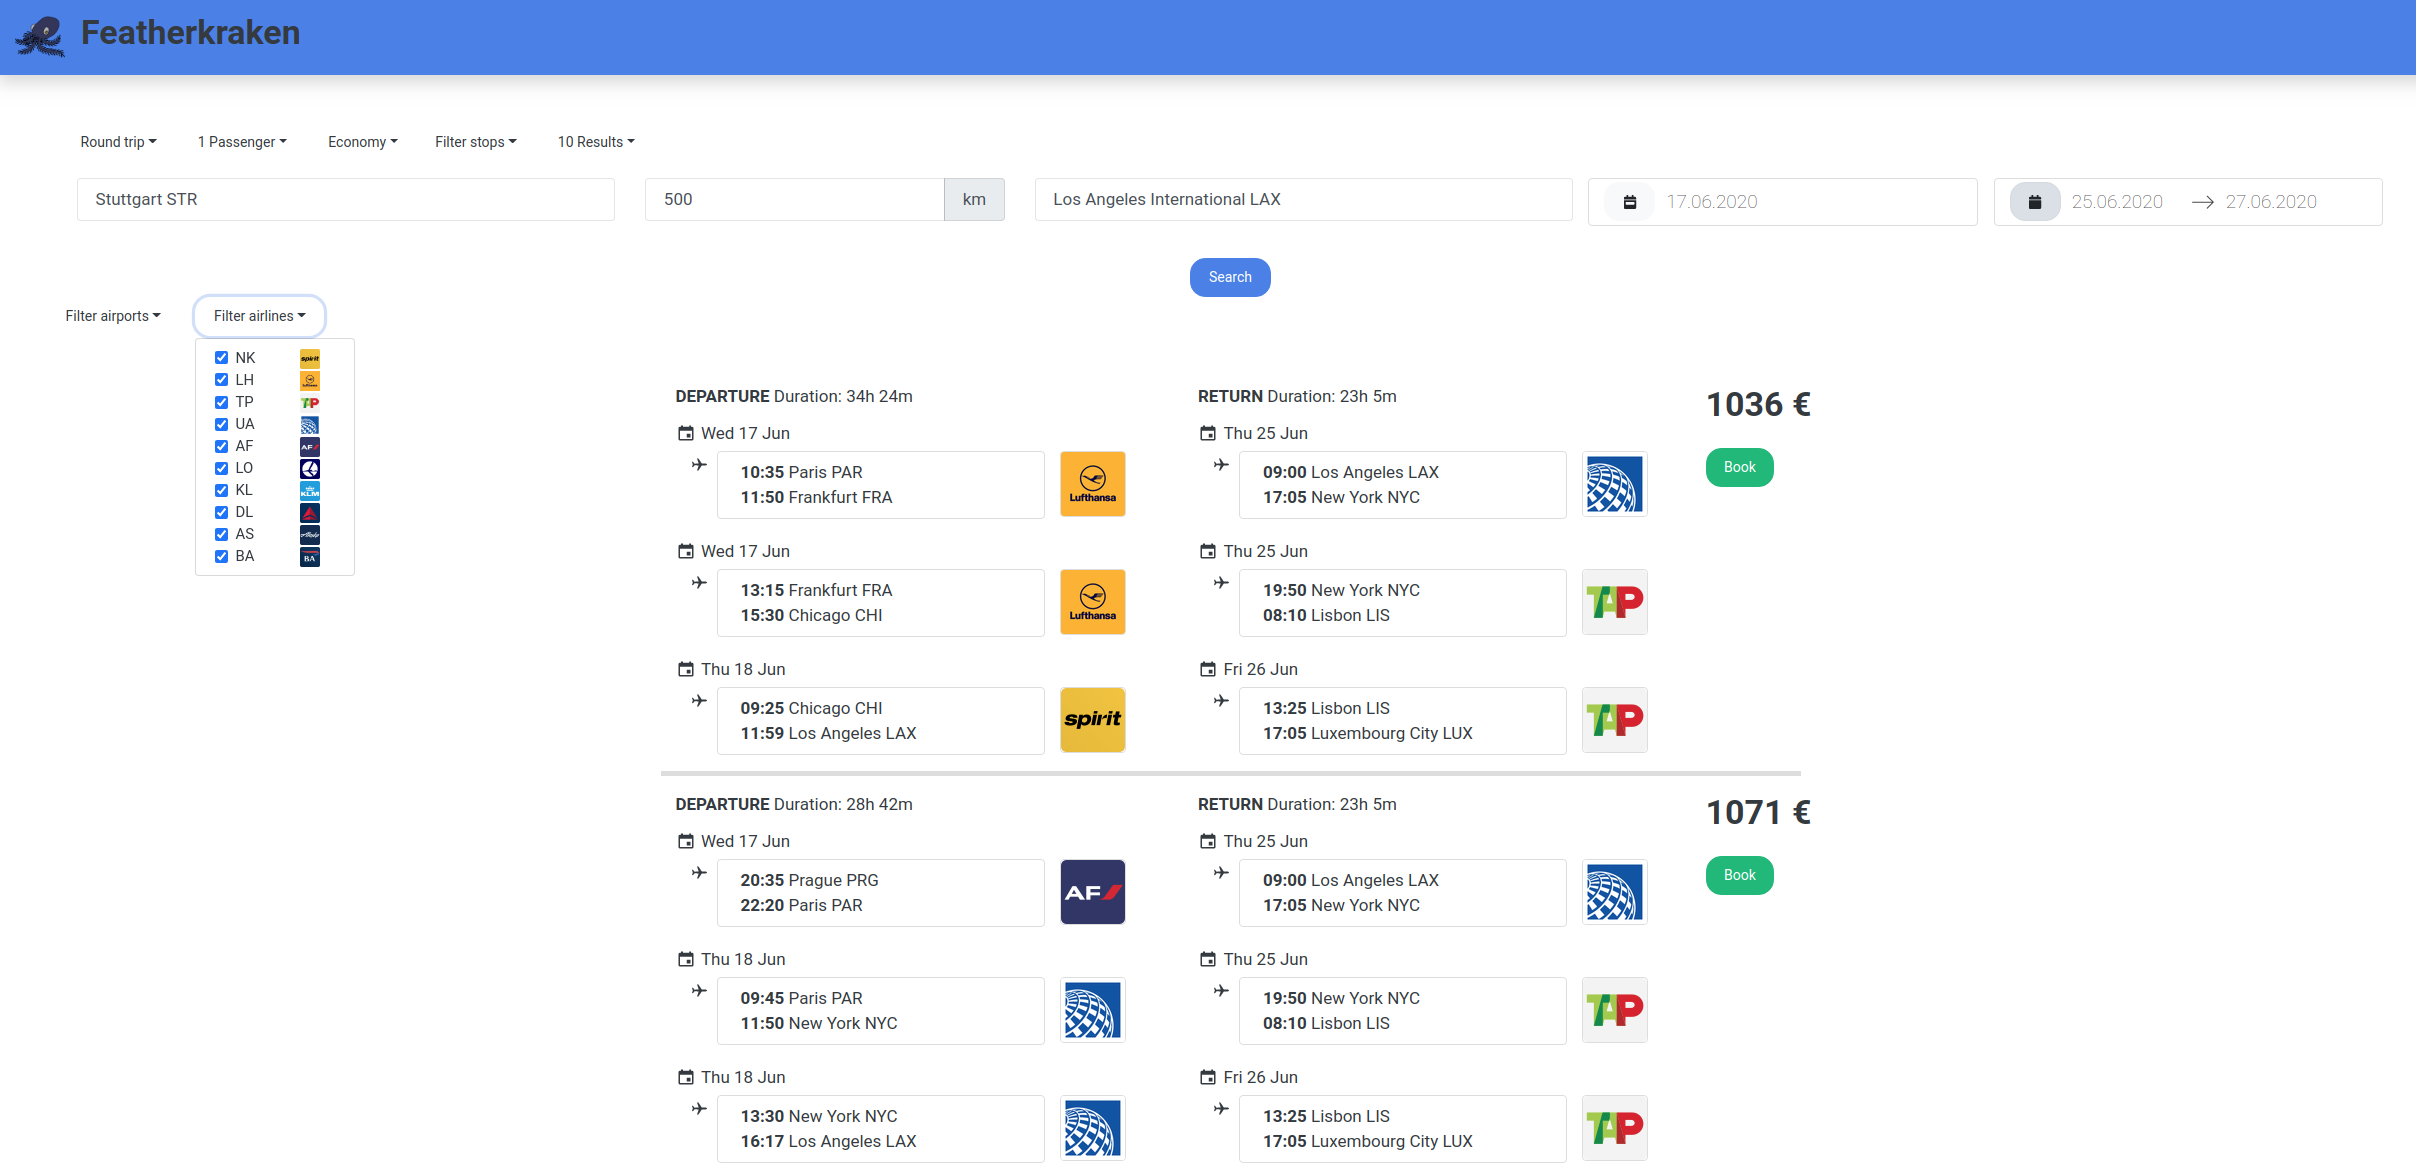
\includegraphics[width=\textwidth]{images/frontend-screenshot}
	\captionof{figure}{Screenshot des Frontend}
	\label{fig:frontend}
\end{center}
Anschließend werden zunächst die Suchfilter in den Dropdowns der ersten Zeile in Abbildung \ref{fig:frontend} erläutert. Zum einen kann nach Art des Fluges (nur Hinflug oder Hin- und Rückflug) gefiltert werden. Ist nur Hinflug ausgewählt, wird das Feld für das Rückreisedatum nicht dargestellt. Über das zweite Dropdown kann die Anzahl erwachsener Passagiere ausgewählt werden. Daneben kann man die gewünschte Klasse (Economy, Premium Economy, Business, First class) angeben und ob man Ergebnisse, die geringere Klassen enthalten, suchen will. Die Auswahl zur Anzahl der Zwischenstopps bietet die Optionen beliebig viele Stops, Non-Stop und bis zu ein oder zwei Stops. Im letzten Dropdown kann man die gewünschte Anzahl der Suchergebnisse auswählen.\\
In den Eingabefeldern darunter können Suchparameter wie Startflughafen, Entfernungsfilter, Zielflughafen und An- und Abreisedatum eingegeben werden. Die Eingabefelder für Start- und Zielflughafen benutzen den Service zur Flughafensuche\textsuperscript{\ref{sec:airport-search}} um Flughäfen mit dem eingegebenen Wortteil in Echtzeit zu suchen. Ist das Feld für den Entfernungsfilter leer oder null wird nur von dem angegebenen Flughafen gesucht. Die Felder für das An- und Abreisedatum können mit Klick auf das Kalender-Icon zwischen klassisch und flexibel wechseln. In Abbildung \ref{fig:frontend} kann man sehen, dass das Abreisedatum fest auf einen Tag und das Abreisedatum dahingegen auf eine Zeitspanne gesetzt ist.\\
Liefert das Backend nach Klicken des Suchbuttons Suchergebnisse zurück, lassen sich diese nach bestimmten Flughäfen und Airlines filtern. Letzteres ist an dem Dropdown auf dem Screenshot beispielhaft zu sehen.\\
Die Suchergebnisse sind in einer Liste aufgeführt und unterteilen sich jeweils in Hin- und Rückflug, wenn nicht nur nach Hinflug gesucht wurde. Alle Informationen über den Flug wie Flugdauer, Start- und Landezeiten und Klasse werden dargestellt. Außerdem informiert ein Logo den Benutzer über die Airline des jeweiligen Flugs.
\newpage
\section{Testing}
Das Testen der Anwendung war ein wichtiger Teil für den Erfolg des Projekts. Deshalb wurden nicht nur alle Software-Komponenten mit Unit-Tests abgedeckt, sondern auch Integrations-Tests geschrieben. All diese Tests werden programmatisch ausgeführt und werden von einer \acrshort{ci} in GitHub automatisch bei jedem \textit{push} ausgeführt. Ein \textit{merge} in den Master ist nur möglich wenn alle Tests erfolgreich ausgeführt wurden. Für alle Testfälle wurden realitätsnahe Bedingungen und Daten gewählt.\\
Zu guter Letzt wurden die Rest-Schnittstelle und die Oberfläche mit der Erwartung der gewünschten Ergebnisse regelmäßig manuell getestet und abgeglichen.
\subsection{Automatische Tests}
Das Java-Backend wurde mit Unit- und Integrationstests getestet, welche mit dem Testframework JUnit 5 geschrieben wurden. Dadurch fallen neue Bugs schon direkt bei der Entwicklung auf. Des Weiteren wird die Qualität des Codes mit \textit{Sonar} überprüft. Dazu zählen unter anderem Aspekte wie Bugs, Schwachstellen (\textit{Vulnerabilities}) oder Verletzung von Java-Richtlinien (sogenannte \textit{Code Smells}). Um Schwachstellen in externen Bibliotheken der Anwendung aufzudecken wird \textit{OWASP} verwendet.\\
All diese Tests werden automatisch in der \acrfull{ci} von \textit{CircleCI} ausgeführt, wenn die Änderungen in das GitHub Repository gepusht werden. Pull Requests sind so konfiguriert, dass sie nur nach erfolgreichem Durchlauf der Tests akzeptiert werden können. Außerdem wird die Testabdeckung bei jedem Durchlauf dokumentiert und überprüft und darf niemals abnehmen. Die Konfiguration dieser Überprüfungen kann dem Dokument \href{https://github.com/featherkraken/featherkraken/blob/master/.circleci/config.yml}{\texttt{featherkraken/.circleci/config.yml}} entnommen werden.\\
Die Komponenten des React.js-Frontends wurden aus Zeitgründen nicht mit automatischen Tests abgedeckt, jedoch wird die Kompilierbarkeit der Anwendung in \textit{CircleCI} überprüft und der Stand des \textit{master}-Branches in GitHub Pages automatisch veröffentlicht. Dies kann in \href{https://github.com/featherkraken/featherkraken-ui/blob/master/.circleci/config.yml}{\texttt{featherkraken-ui/.circleci/config.yml}} eingesehen werden.
\subsection{Manuelle Tests}
Zusätzlich zu den automatischen Tests gibt es eine \textit{Postman-Collection}\textsuperscript{\ref{sec:postman}} für die Rest-Schnittstellen des Backends. Diese kann unter \href{https://github.com/featherkraken/featherkraken/blob/master/src/test/postman/Collection.json}{\texttt{src/test/postman/Collection.json}} gefunden und in \textit{Postman} importiert werden. Diese Anfragen wurden regelmäßig bei der Entwicklung des Backends verwendet, um Fehlerursachen zu finden und die Funktion sicherzustellen.\\
Außerdem gibt es Testfälle für das Frontend, um die Umsetzung der Anwendung mit den tatsächlichen Anforderungen vergleichen zu können. Folgend sind einige dieser Testfälle aufgeführt:
\vspace{1cm}
\begin{center}
	\captionsetup{type=figure}
	\resizebox{\textwidth}{!}
	{\begin{tabular}{ l | l | l | l }
			\textbf{Abflughafen} & \textbf{Zielflughafen} & \textbf{Klasse} & \textbf{Erwartung} \\
			\hline
			Inverness INV & John F. Kennedy International JFK & First class &  Umstieg mit Economy Klasse wird gefunden\\
			\hline
			Heathrow LHR & John F. Kennedy International JFK & First class &  Flüge werden gefunden\\
			\hline
			Munich MUC (+600km) & Kyiv International Airport (Zhuliany) IEV & Economy &  Flug von LEJ gefunden\\
			\hline
			Stockholm Arlanda ARN & Dubai International DXB & First class &  Umstieg mit Business Klasse wird gefunden\\
			\hline
			Sofia SOF & San Francisco International & Business &  Umstieg mit Economy wird gefunden\\
	\end{tabular}}
	\captionof{figure}[Testfälle des Frontends]{Tabelle für die Testfälle des Frontends}
	\label{fig:ui-tests}
\end{center}
\newpage
% Ende
\section{Fazit}
In diesem Kapitel wird zunächst in einem Ausblick auf Möglichkeiten zur Verbesserung der Anwendung eingegangen, denn Software-Entwicklung ist ein niemals abgeschlossener Vorgang. Alle Punkte sind in GitHub Issues festgehalten, sodass sie nicht in Vergessenheit geraten können. Zum Abschluss wird das gesamte Projekt noch einmal zusammengefasst.
\subsection{Ausblick}
Um die Funktion der Anwendung zu erweitern, könnte man zum Beispiel weitere externe Schnittstellen anbinden, um eventuell billigere Flüge als die von Kiwi.com zu finden. Dazu wurden die betroffenen Klassen des Java-Backends schon so abstrakt geschrieben, sodass dies mit angemessenen Aufwand umsetzbar ist.\\
Dabei ist jedoch anzumerken, dass diese externen Aufrufe bist jetzt nicht asynchron erfolgen. Das heißt, dass gewartet wird bis alle externen Schnittstellen geantwortet haben. Das hat zur Folge, dass die Antwortzeit äquivalent zur langsamsten Schnittstelle ist. Um das zu ändern, muss zunächst evaluiert werden, ob diese asynchron beantwortet werden können.\\
Als weitere Verbesserung kann die Geschwindigkeit der Aufrufe dokumentiert werden. Damit kann entschieden werden, ob bestimmte externe Schnittstellen zu langsam sind und damit wieder entfernt werden sollten. Für diese Art von Monitoring gibt es bereits Lösungen wie \href{https://prometheus.io/}{\textit{Prometheus}} oder die eingebaute Funktion von Eclipse Microprofile mithilfe sogenannter \textit{Metrics}.\\
Des Weiteren kann auch ein Entfernungsfilter für den Zielflughafen auf die selbe Art wie für den Startflughafen hinzugefügt werden. Dazu müsste das Backend und die Oberfläche angepasst werden. Da dies jedoch nicht im Fokus der Aufgabe stand, sei das jedoch nur als Idee anzumerken.\\
Es wurde versucht, das Java-Backend auf \href{https://www.heroku.com/}{\textit{Heroku}} zu hosten, damit sie jederzeit im Internet genutzt werden kann. Dies war aber selbst nach vielen Tagen nicht nachvollziehbar, also wurde dieser Ansatz verworfen. Als Zwischenlösung könnte die Anwendung auf einem Linux-Server bereitgestellt werden. Dies sollte automatisch mit jeder Änderung im GitHub Repository erfolgen, wie es mit \textit{Heroku} versucht wurde.
\subsection{Zusammenfassung}
Nachdem die Aufgabenstellung evaluiert wurde, konnte schrittweise eine Softwarelösung entworfen werden. Dabei wurden verschiedene Abstraktionsebenen des Problems betrachtet und jeweilige Lösungen gefunden. Mit den gewählten Technologien wurde eine Webanwendung und eine Serveranwendung entwickelt, welche sich durch hohe Plattformunabhängigkeit auszeichnen. Es wurde darauf geachtet, dass die Anwendung leicht erweitert werden kann und der Code verständlich ist. Die Anwendungen werden mit \acrfull{ci} automatisch getestet und im Falle der Webanwendung auch immer mit dem neuesten Stand im Internet veröffentlicht. Abschließend wurde ein Ausblick auf Verbesserungsmöglichkeiten und Ansätze dafür aufgeführt.
\end{sloppypar}
% Literaturverzeichnis
\newpage
% set interlinepenalty to not split entries on page break
\bibliographystyle{apacite}
\bibliography{paper}
\end{document}